% ==============================================================================
% sec:historie --- Historický vývoj
% ==============================================================================
% Zdroje: Pokorny_HistorieOdbory2020, Pokorny_100letMOP2019,
%         Hala_SystemySocialnihoDialogu2013, Weber_Industrie40_2015
%         Casale_SocialDialogueCzechSuccessStory2001
% ==============================================================================

Vznik odborového hnutí je neoddělitelně spjat s~průmyslovou revolucí 19.~století.
Mechanizace výroby vedla k~hromadné koncentraci pracovní síly v~továrnách, k~prodlužování pracovní doby a~ke zhoršování pracovních podmínek, na~něž zaměstnanec jako jednotlivec neměl prostředky jak reagovat.
Kolektivní organizace zaměstnanců se~v~tomto kontextu ustavily jako reakce na~strukturální asymetrii vyjednávací síly mezi vlastníkem kapitálu a~námezdním pracovníkem.\par
Industrializace v~křehkém mnohonárodnostním Rakousku--Uhersku byla provázena progresivními sociálními zákony, které navazovaly na reformy feudalismu a~merkantilismu po Napoleonských válkách -- regulace dětské práce (univerzální školní docházka 1774) a~lokálního poddanství (robotní patent 1781). Po ekonomické krizi a~následných revolučních událostech roku 1848 došlo ke zrušení poddanství a~oslabení cechovních struktur, což vedlo k~volnému pohybu práce a~spolu s~technologickým pokrokem urychlilo rozvoj průmyslu.
V~českých zemích se~první větší kolektivní akce datují do~druhé poloviny 19.~století. Mezi charakteristické události patří stávka pražských typografů v~roce 1869, jež skončila uvězněním účastníků, ale zároveň prosazením vyšších mezd; a~hornická stávka na~Nýřansku v~roce 1882, která propojila zaměstnance napříč doly téhož revíru, a~která byla krvavě potlačena. Sdružování v~odborových organizacích a~kolektivní akce legalizoval v~roce 1870 koaliční zákon (\emph{Koalitionsgesetz}). Spolu se stávkovými směrnicemi rakouských odborů (\emph{Streikreglement}, 1894) se stávka ze vzpoury proměnila v~regulovaný nástroj sociálního dialogu, který tak probíhal zejména za účelem udržování sociálního smíru.~\cite{Pokorny_HistorieOdbory2020}\par
Právě Typografická beseda, dohoda pražských typografů s~tiskárnami z~roku~1864 a~pozdější vysoké pokrytí \aclpins{KS} v~grafickém průmyslu ukazují, že~základy kultivovaného, nenásilného sociálního dialogu v~českých zemích byly položeny tam, kde se~kvalifikovaná práce dokázala organizačně opřít o~profesní identitu, čitelné mzdové nároky a~vnitřní solidaritu. Pro současnou debatu z~toho plyne, že sociální dialog nemůže být rámován pouze jako ochrana nejzranitelnějších zaměstnanců, ale musí získávat aktivní podporu také mezi vysoce kvalifikovanými profesemi, protože právě ony v~technologicky zlomových obdobích určují standard práce a~legitimitu kolektivního vyjednávání.\par

\begin{figure}[H]
    \centering
    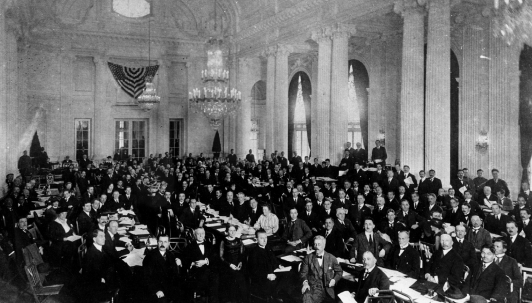
\includegraphics[width=\linewidth]{../pics/ILO.png}
    \caption{První mezinárodní konference práce \acs{MOP} ve Washingtonu v~roce 1919. Převzato z~\cite{Pokorny_100letMOP2019}.}
    \label{fig:ILO}
\end{figure}

Klíčovým momentem ukotvení pracovního práva v~mezinárodním měřítku bylo v~roce 1919 založení \acgen{MOP} jako součásti Versailleského mírového systému.
\Ac{MOP} se~jako jediná specializovaná mezinárodní organizace Společnosti národů, posléze \acf{OSN}, opírá o~tripartitní princip -- na~jejím rozhodování se~rovnocenně podílejí zástupci vlád, zaměstnavatelů a~zaměstnanců.
Československá republika patřila k~zakládajícím členům \acgen{MOP} a~na~Washingtonskou konferenci v~roce 1919 vyslala delegaci, v~níž zaměstnaneckou stranu zastupoval Rudolf Tayerle, pozdější člen Správní rady \acgen{MOP}. Technickou a~politickou podporu zaměstnavatelům v~\acloc{MOP} zprostředkovává \acf{IOE} založená v~roce 1920, jejímž zakládajícím členem byl také Ústřední svaz československých průmyslníků.\par
Meziválečné odborové hnutí navazovalo zejména v~Čechách na~rakousko-uherskou tradici prostřednictvím vyspělé sítě odborových centrál a~politicky etablovaných sociálnědemokratických struktur. V~porevolučním období v~roce 1920 bylo uzavřeno vrcholných 1~259 kolektivních smluv pokrývajících téměř milion zaměstnanců ve 46~802 podnicích. Ve výrobě strojů se silnou odborovou tradicí dosahovalo pokrytí \aclpins{KS} \SI{96}{\percent} zaměstnanců. Také Baťa vnímal -- po vzoru USA -- sociální dialog a~transparentní systém odměňování, benefitů a~vzdělávání jako nástroj k~dosažení vysoké produktivity práce.\par
Již krátce po~vzniku republiky byl přijat zákon č.~91/1918~Sb.,\ o~osmihodinové pracovní době, jenž o~několik měsíců předběhl Úmluvu \acgen{MOP} č.~1 a~stal se~jedním z~prvních zákonů svého druhu v~Evropě. Navazovaly zákony č.~144/1920~Sb.\ a~č.~330/1921~Sb.~o~závodních výborech, které měly spolupůsobit při uzavírání \acfpgen{KS} a~kontrolovat jejich plnění; nicméně právní závaznost \acpgen{KS} nebyla do hospodářské krize na přelomu 20.\ a 30.~let zákonem stanovena. V~roce 1935 překročil počet pracujících organizovaných v~československých odborech 2~mil.~členů, v~českých zemích dosáhla odborová organizovanost zhruba \SI{50}{\percent}.\par
Důsledkem pokrizového zhoršování pracovních podmínek bylo Československo zmítáno velkými stávkami v~uhelných revírech, které byly násilně potlačovány (Duchcovská, Frývaldovská, Mostecká). Narůstající potřeba stabilizace společnosti i~ve světle německé hrozby vedla k~legislativnímu posílení \aclgen{KV}. Kolektivní smlouvy byly znovu silněji vnímány jako smluvní alternativa k~stávkové konfrontaci. Vládní nařízení prodlužovala platnost \acpgen{KS} (č.~118/1934~Sb.), určovala nadřazenost \acpgen{KS} nad individuálními smlouvami (č.~89/1935~Sb.), rozšiřovala regionálně závaznost odvětvových \acgen{KS} v~textilním průmyslu (č.~102/1935~Sb.) a~konečně obecně stanovovala postup pro rozšiřování závaznosti \acpgen{KS} v~regionech a~odvětvích (č.~141/1937~Sb.).
Tento vývoj byl ukončen nacistickou okupací, kdy byly nezávislé odbory likvidovány a~kolektivní smlouvy nahrazeny mzdovými vyhláškami okupační moci, a~následně zásadně transformovány poúnorovým režimem.\par

Komunistický režim převedl oslabené odborové hnutí pod jednotnou organizační strukturu \acgen{ROH}, které podle režimu v~novém společenském uspořádání nemělo před kým hájit zájmy pracujících, dohled nad blahobytem byl převeden na státní instutuce a~odbory místo toho zprostředkovávaly převodní funkci mezi stranou a~pracovištěm, distribuci sociálních benefitů a~mobilizaci pracovní síly. Organizace zaměstnavatelů byly rozpuštěny.
\Ac{ROH} z~podstaty nemohlo plnit funkci nezávislého kolektivního vyjednavače, neboť stát i~zaměstnavatel byli totéž a~mzdový tarif byl stanovován centrálně. Právo na~stávku nebylo v~ústavě uznáno (za což bylo Československo v~\acloc{MOP} kritizováno) a~kolektivní akce zaměstnanců byly v~praxi vyloučeny, s~výraznou výjimkou hornických a~plzeňských stávek proti měnové reformě v~létě 1953 a~protestů proti sovětské okupaci v~roce 1968.
Důsledkem této čtyřicetileté zkušenosti je v~\acsloc{ČR} přetrvávající nedůvěra k~\aclpdat{OO}, která tvoří bariéru i~pro současné nezávislé odbory s~odlišným právním a~organizačním ukotvením.~\cite{Pokorny_HistorieOdbory2020}~\cite{Pokorny_100letMOP2019}\par

Transformace po~roce 1989 přinesla obnovení svobody sdružování i~moderní zákonný rámec \aclgen{KV}.
V~roce 1990 vznikla \acf{ČMKOS} jako nová zastřešující centrála nezávislých \aclpgen{OS} a~Koordinační rada podnikatelských svazů a~sdružení \acs{ČR}, pojmenovaná od roku 1993 \acf{KZPS}. Právním základem pro organizaci sociálních partnerů se stal zákon č.~83/1990~Sb., o~sdružování občanů, dnes nahrazený novým občanským zákoníkem. S~obnovou sociálního dialogu v~postkomunistických zemích vypomáhala \ac{MOP} expertními misemi. Nová legislativa ratifikovala Úmluvu č.~87, o~svobodě sdružování a~ochraně práva odborově se organizovat z~roku 1948, a~Úmluvu č.~98, o~právu organizovat se a~kolektivně vyjednávat z~roku 1949, a~implementovala pozdější Úmluvu č.~135, o~zástupcích zaměstnanců. Principy rozšíření závaznosti \acpgen{KS} byly inspirovány meziválečnou legislativou a~Úmluvou č.~154, o~kolektivním vyjednávání. Naopak správa nemocenských a~rodinných dávek byla odborům odňata. V~roce 1991 byl přijat zákon č.~2/1991~Sb.,\ o~kolektivním vyjednávání, a~současně byla založena \ac{RHSD} na půdorysu Úmluvy č.~144, o~tripartitních jednáních, jako dobrovolné fórum koordinace zájmů sociálních partnerů a~vlády. Generální dohody uzavírané v~letech 1991--1994 v~rámci tripartity kupříkladu napomohly se stabilizací inflace koordinací růstu mezd (omezení do \SI{5}{\percent} meziročně).
Legislativní rámec se~tak rychle dostal na~úroveň srovnatelnou se~zeměmi vznikající \aclgen{EU}, praxe sociálního dialogu v~následujících letech však s~tímto rámcem nedržela krok.\par

Zatímco na~konci 80.~let bylo organizováno v~odborech přes \SI{80}{\percent} zaměstnanců (skrze \ac{ROH}), v~roce 2025 se~odborová organizovanost pohybuje kolem \SI{10}{\percent}.
Pokles členství po roce 1989 je výsledkem privatizace a~rozdělení velkých státních podniků, individualismu -- a~to nejen v~pracovních vztazích, nedůvěry v~odbory zděděné po~\acloc{ROH} a~celkového negativního vnímání odborů jako přežitku minulého režimu.
Zaměstnavatelské svazy sdružují pouze malou část právnických osob (cca \SI{6}{\percent}), které ale zaměstnávají asi \SI{60}{\percent} zaměstnanců.
V~roce 1995 se z~\acgen{KZPS} oddělil \ac{SPČR} s~přibližně polovinou zaměstnanců zejména ve velkých průmyslových podnicích a~vznikla \ac{ASO}, čímž došlo k~zvýšení počtu subjektů v~tripartitě. Práh reprezentativity zástupců zaměstnanců se v~roce 2000 snížil ze 200~tis.~členů na 150~tis., přesto zastoupení v~\acloc{RHSD} pozbyla Konfederace umění a~kultury (KUK); naopak u~zástupců zaměstnavatelů došlo postupně ke zvýšení prahu ze 100~tis.~zaměstnanců na 400~tis.~zaměstnanců.
Formální struktura sociálního dialogu byla dosud zachována, jeho faktický dosah je však slabý -- pokrytí pracovněprávních vztahů \aclpins{KS} dlouhodobě dosahuje pouze přibližně \SI{30}{\percent}, což \acacc{ČR} řadí mezi země s~nejnižším pokrytím v~rámci celé \acsgen{EU}.\par
V~postkomunistickém neoliberálním politickém prostředí zaštiťovaném ochranou majetkových práv a~negativní svobodou sdružování, tedy práva nebýt organizován ani vázán cizími \acpins{KS} na odvětvové úrovni (v~rámci institutu rozšiřování platnosti \aclpgen{KSVS}), chybí dlouhodobý závazek vlád k~podpoře sociálního dialogu a~tripartita byla opakovaně marginalizována na nástroj udržení sociálního smíru v~krizích.
Tento přístup ke sdružování poškodil také členství v~zaměstnavatelských svazích a~vedl k~jejich nízké reprezentativitě vůči malým podnikům a~živnostníkům. Sociální dialog se tak rozvinul zejména na podnikové úrovni.\par
V~rámci evropského společenství je \acl{ČR} spíše zdrženlivá při implementaci mezinárodních smluv posilující moderní pracovní právo -- v~90.~letech Evropské sociální charty (\acs{ČR} dosud není ani signatářem revize z~roku 1996) nebo aktuálně směrnic \acs{EU} o~přiměřených minimálních mzdách a~o~transparentním odměňování.\par

Úroveň otevřené konfliktnosti mezi sociálními partnery je v~\acloc{ČR} v~evropském srovnání nízká. V~90.~letech navzdory rázným reformám, které provázela ekonomická nestabilita a~hospodářská kriminalita, spojeným s~propadem životní úrovně značné části obyvatelstva (v~roce 1991 kupní síla poklesla o~\SI{26}{\percent} zatímco produktivita práce o~\SI{7}{\percent}), byl v~podnicích udržen sociální smír tak, že nebyl narušen přechod k~tržnímu hospodářství, ani~příliv zahraničního kapitálu. Ve zbytku 90.~let reálné mzdy ztrátu dorovnaly a~po roce 1995 do roku 2000 překonávaly, což přispělo k~relativní stabilitě sociálního dialogu. Tato stabilita přispěla ke vzniku nové legislativy ochraňující zaměstnance před insolvencí zaměstnavatelů a~na přelomu tisíciletí k~úspěšné harmonizaci legislativy před vstupem do \acs{EU} v~roce 2004.\par
Pro společnost nejviditelnější polistopadová činnost odborů je politická a~je spojena se~čtyřmi vlnami reformních zásahů pravicových vlád -- v~roce 1994 petice s~600~tis.\ podpisy, demonstrace a~generální stávka s~účastí téměř 1,5~milionu zaměstnanců, které byly reakcí na~reformní zásahy první Klausovy vlády do~důchodového systému a~zákoníku práce; 8.~listopadu~1997 demonstrace proti úsporným balíčkům druhé Klausovy vlády (která následně kvůli kauze rozsáhlé privatizační korupce padla), jíž se~zúčastnilo přibližně 100\,000 osob; v~letech 2007--2008 výstražná stávka ve~zdravotnictví proti Julínkově reformě (privatizace zdravotních pojišťoven a~nemocnic) a~protesty „Děkujeme, odcházíme”, „Stop vládě” a~v~letech 2010--2012 stávka v~dopravě proti podfinancování zdravotnictví a~reformnímu balíčku Nečasovy vlády s~obdobnou účastí.
Naposledy v~roce 2023 proběhla jednodenní výstražná stávka ve školství proti ozdravnému balíčku Fialovy vlády (snižování rozpočtu na nepedagogické pracovníky škol, omezení zaměstnaneckých benefitů, úprava penzijního systému), doprovázená hodinovou stávkou v~průmyslu.~\cite{Hala_RozvojSocialnihoDialoguCR2002}~\cite{Casale_SocialDialogueCzechSuccessStory2001}\par

Současný kontext digitalizace, robotizace a~rozvoje umělé inteligence představuje pro evropský trh práce nový industrializační impuls, jehož dopady jsou přirovnávány k~přechodu k~průmyslové výrobě v~19.~století.
Obnovení silného \aclgen{KV} zajišťujícího udržitelnost potenciálních strukturálních změn v~\acsloc{ČR} předpokládá překonání historicky ukotvených bariér -- ztráty důvěry v~odbory, nízké reprezentativnosti zaměstnavatelských svazů v~rámci sociálního dialogu, vnímání sociálního dialogu jako brzdy hospodářského rozvoje a~nevyužití polistopadového formálního rámce \aclgen{KV}.\par
